% Options for packages loaded elsewhere
\PassOptionsToPackage{unicode}{hyperref}
\PassOptionsToPackage{hyphens}{url}
\PassOptionsToPackage{dvipsnames,svgnames,x11names}{xcolor}
%
\documentclass[
]{book}
\usepackage{amsmath,amssymb}
\usepackage{iftex}
\ifPDFTeX
  \usepackage[T1]{fontenc}
  \usepackage[utf8]{inputenc}
  \usepackage{textcomp} % provide euro and other symbols
\else % if luatex or xetex
  \usepackage{unicode-math} % this also loads fontspec
  \defaultfontfeatures{Scale=MatchLowercase}
  \defaultfontfeatures[\rmfamily]{Ligatures=TeX,Scale=1}
\fi
\usepackage{lmodern}
\ifPDFTeX\else
  % xetex/luatex font selection
  \setmonofont[Scale=0.775]{MesloLGS NF}
\fi
% Use upquote if available, for straight quotes in verbatim environments
\IfFileExists{upquote.sty}{\usepackage{upquote}}{}
\IfFileExists{microtype.sty}{% use microtype if available
  \usepackage[]{microtype}
  \UseMicrotypeSet[protrusion]{basicmath} % disable protrusion for tt fonts
}{}
\makeatletter
\@ifundefined{KOMAClassName}{% if non-KOMA class
  \IfFileExists{parskip.sty}{%
    \usepackage{parskip}
  }{% else
    \setlength{\parindent}{0pt}
    \setlength{\parskip}{6pt plus 2pt minus 1pt}}
}{% if KOMA class
  \KOMAoptions{parskip=half}}
\makeatother
\usepackage{xcolor}
\usepackage{longtable,booktabs,array}
\usepackage{calc} % for calculating minipage widths
% Correct order of tables after \paragraph or \subparagraph
\usepackage{etoolbox}
\makeatletter
\patchcmd\longtable{\par}{\if@noskipsec\mbox{}\fi\par}{}{}
\makeatother
% Allow footnotes in longtable head/foot
\IfFileExists{footnotehyper.sty}{\usepackage{footnotehyper}}{\usepackage{footnote}}
\makesavenoteenv{longtable}
\usepackage{graphicx}
\makeatletter
\def\maxwidth{\ifdim\Gin@nat@width>\linewidth\linewidth\else\Gin@nat@width\fi}
\def\maxheight{\ifdim\Gin@nat@height>\textheight\textheight\else\Gin@nat@height\fi}
\makeatother
% Scale images if necessary, so that they will not overflow the page
% margins by default, and it is still possible to overwrite the defaults
% using explicit options in \includegraphics[width, height, ...]{}
\setkeys{Gin}{width=\maxwidth,height=\maxheight,keepaspectratio}
% Set default figure placement to htbp
\makeatletter
\def\fps@figure{htbp}
\makeatother
\setlength{\emergencystretch}{3em} % prevent overfull lines
\providecommand{\tightlist}{%
  \setlength{\itemsep}{0pt}\setlength{\parskip}{0pt}}
\setcounter{secnumdepth}{5}
\usepackage{amsmath}
\usepackage{amssymb}
\usepackage{amsfonts}

\defaultfontfeatures{Scale=MatchLowercase}

\usepackage{booktabs}
\usepackage{longtable}
\usepackage[bf,singlelinecheck=off]{caption}

\usepackage{framed,color}
\definecolor{shadecolor}{RGB}{248,248,248}

\renewcommand{\textfraction}{0.05}
\renewcommand{\topfraction}{0.8}
\renewcommand{\bottomfraction}{0.8}
\renewcommand{\floatpagefraction}{0.75}

\renewenvironment{quote}{\begin{VF}}{\end{VF}}
\let\oldhref\href
\renewcommand{\href}[2]{#2\footnote{\url{#1}}}

\ifxetex
  \usepackage{letltxmacro}
  \setlength{\XeTeXLinkMargin}{1pt}
  \LetLtxMacro\SavedIncludeGraphics\includegraphics
  \def\includegraphics#1#{% #1 catches optional stuff (star/opt. arg.)
    \IncludeGraphicsAux{#1}%
  }%
  \newcommand*{\IncludeGraphicsAux}[2]{%
    \XeTeXLinkBox{%
      \SavedIncludeGraphics#1{#2}%
    }%
  }%
\fi

\makeatletter
\newenvironment{kframe}{%
\medskip{}
\setlength{\fboxsep}{.8em}
 \def\at@end@of@kframe{}%
 \ifinner\ifhmode%
  \def\at@end@of@kframe{\end{minipage}}%
  \begin{minipage}{\columnwidth}%
 \fi\fi%
 \def\FrameCommand##1{\hskip\@totalleftmargin \hskip-\fboxsep
 \colorbox{shadecolor}{##1}\hskip-\fboxsep
     % There is no \\@totalrightmargin, so:
     \hskip-\linewidth \hskip-\@totalleftmargin \hskip\columnwidth}%
 \MakeFramed {\advance\hsize-\width
   \@totalleftmargin\z@ \linewidth\hsize
   \@setminipage}}%
 {\par\unskip\endMakeFramed%
 \at@end@of@kframe}
\makeatother

\renewenvironment{Shaded}{\begin{kframe}}{\end{kframe}}

\usepackage{makeidx}
\makeindex

\urlstyle{tt}

\usepackage{amsthm}
\makeatletter
\def\thm@space@setup{%
  \thm@preskip=8pt plus 2pt minus 4pt
  \thm@postskip=\thm@preskip
}
\makeatother

\DeclareMathOperator{\E}{\mathbb{E}} % Define ev operator
\DeclareMathOperator{\V}{\mathbb{V}} % Define variance operator
\DeclareMathOperator{\Var}{\mathbb{V}} % Define variance operator
\DeclareMathOperator{\SD}{SD} % Define sd operator
\DeclareMathOperator{\Cov}{Cov} % Define covariance operator
\DeclareMathOperator{\Corr}{Corr} % Define correlation operator
\DeclareMathOperator{\Me}{Me} % Define mediane operator
\DeclareMathOperator{\Mo}{Mo} % Define mode operator

\DeclareMathOperator{\Bin}{Binomial} % Define binomial operator
\DeclareMathOperator{\Bernoulli}{Bernoulli} % Define Bernoulli operator
\DeclareMathOperator{\Ber}{\mathscr{B}} % Define Bernoulli operator
\DeclareMathOperator{\Poi}{Poisson} % Define Poisson operator
\DeclareMathOperator{\Uniform}{Uniform} % Define Uniform operator
\DeclareMathOperator{\Cauchy}{Cauchy} % Define Cauchy operator
\DeclareMathOperator{\B}{B} % beta function
% \mbox{B}(a, b) % beta function
% \mbox{Beta}(a, b) % beta distribution

\DeclareMathOperator{\elpd}{elpd} % Define elpd operator
\DeclareMathOperator{\lppd}{lppd} % Define lppd operator
\DeclareMathOperator{\LOO}{LOO} % Define LOO operator
\DeclareMathOperator{\argmin}{arg\,min} 
\DeclareMathOperator{\argmax}{arg\,max} 

\newcommand{\E}{\mathbb{E}} % Define expected value operator
\newcommand{\R}{\textsf{R}} % Define R programming language symbol
\newcommand{\Real}{\mathbb{R}} % Define real number operator
\newcommand{\Prob}{\mathscr{P}}
\newcommand{\indep}{\perp \!\!\! \perp}

\usepackage[
 labelfont=bf,
 font={small, it}
]{caption}
\usepackage{upquote} % print correct quotes in verbatim-environments
\usepackage{empheq}
\usepackage{xfrac}

\usepackage{polyglossia}
\setmainlanguage{italian}

\frontmatter
\ifLuaTeX
  \usepackage{selnolig}  % disable illegal ligatures
\fi
\usepackage[]{natbib}
\bibliographystyle{apalike}
\IfFileExists{bookmark.sty}{\usepackage{bookmark}}{\usepackage{hyperref}}
\IfFileExists{xurl.sty}{\usepackage{xurl}}{} % add URL line breaks if available
\urlstyle{same}
\hypersetup{
  pdftitle={Appunti di Costruzione e validazione di strumenti di misura dell'efficacia dell'intervento psicologico in neuropsicologia -- B020881 (B213)},
  pdfauthor={Corrado Caudek},
  colorlinks=true,
  linkcolor={Maroon},
  filecolor={Maroon},
  citecolor={Blue},
  urlcolor={Blue},
  pdfcreator={LaTeX via pandoc}}

\title{Appunti di Costruzione e validazione di strumenti di misura dell'efficacia dell'intervento psicologico in neuropsicologia -- B020881 (B213)}
\author{Corrado Caudek}
\date{2023-04-22}

\begin{document}
\maketitle

\cleardoublepage\newpage\thispagestyle{empty}\null
% \cleardoublepage\newpage\thispagestyle{empty}\null
%\cleardoublepage\newpage
\thispagestyle{empty}
\begin{center}
\Large{Appunti di Costruzione e validazione di strumenti di misura dell'efficacia dell'intervento psicologico in neuropsicologia -- AA 2021/2022}

\vskip20pt

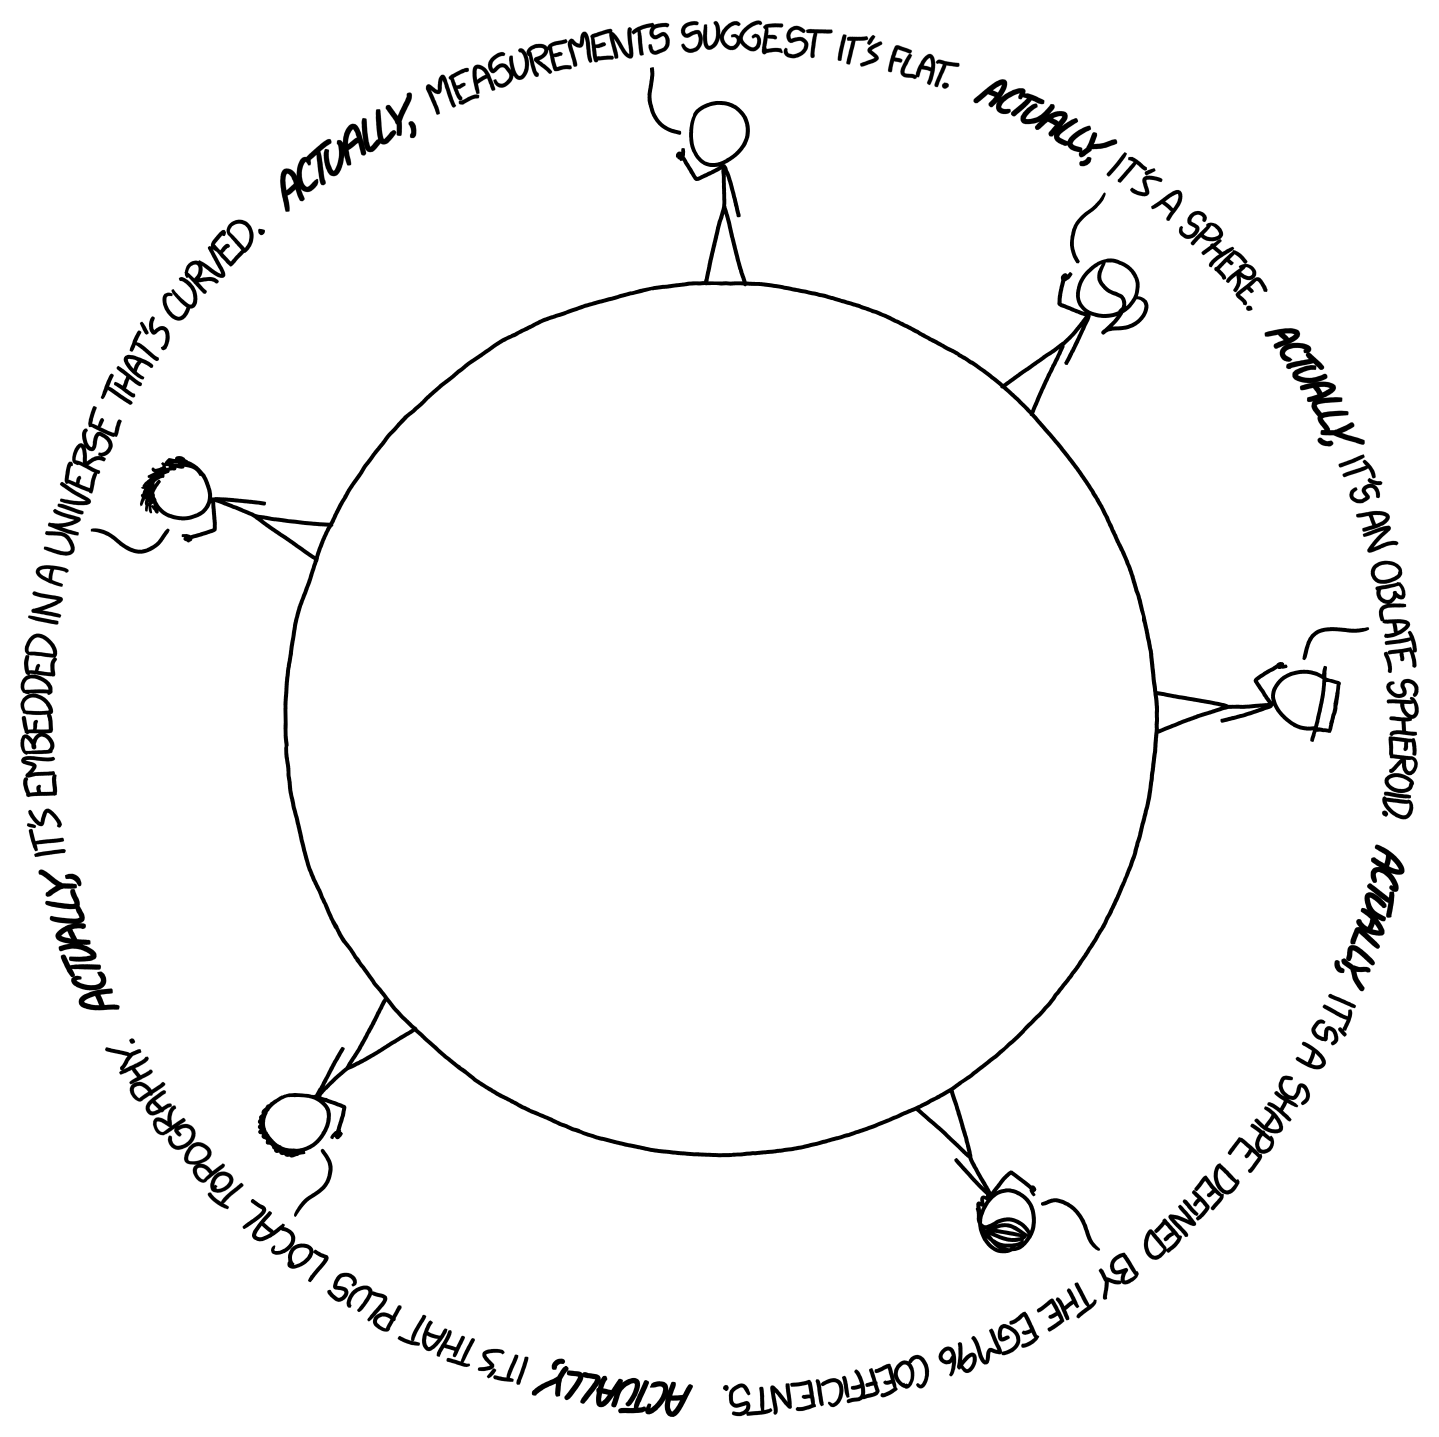
\includegraphics{images/actually_2x.png}
\end{center}

\setlength{\abovedisplayskip}{-5pt}
\setlength{\abovedisplayshortskip}{-5pt}

{
\hypersetup{linkcolor=}
\setcounter{tocdepth}{2}
\tableofcontents
}
\listoffigures
\listoftables
\hypertarget{benvenuti}{%
\chapter*{Benvenuti}\label{benvenuti}}


Benvenuti nella versione online di \emph{Costruzione e validazione di strumenti di misura dell'efficacia dell'intervento psicologico in neuropsicologia}. Questo sito web contiene il materiale didattico dell'insegnamento B020881 (B213) rivolto agli studenti del secondo anno del Corso di Laurea Magistrale in Psicologia Clinica e della Salute e Neuropsicologia (curriculum: assessment e intervento psicologici in neuropsicologia - E21), A.A. 2022-2023. L'insegnamento si propone di fornire agli studenti un'introduzione all'assessment psicologico, ovvero un insieme di conoscenze/competenze che si pongono all'intersezione tra psicometria, statistica e informatica.

L'obiettivo dell'insegnamento sarà concentrato sull'analisi fattoriale esplorativa (EFA) e sulla confermatoria (CFA), che sono gli strumenti principali utilizzati nel processo di sviluppo dei test psicometrici per esaminare la struttura latente di una scala psicologica, ad esempio un questionario. In particolare, la CFA viene utilizzata per determinare il numero di dimensioni sottostanti gli indicatori (fattori) e l'intensità delle relazioni tra gli indicatori e i fattori (saturazioni fattoriali). La CFA è anche utile per comprendere come effettuare lo scoring dei test e per identificare il numero di sottoscale e come queste debbano essere codificate.

Inoltre, la CFA è un importante strumento analitico nella valutazione psicometrica, in quanto consente di stimare l'affidabilità della scala dei test psicometrici, evitando i problemi della teoria classica dei test, ad esempio l'alpha di Cronbach. Con i recenti progressi nell'analisi dei dati categoriali, la CFA offre ora un quadro analitico comparabile a quello offerto dalla teoria di risposta agli item (IRT). In realtà, secondo \citet{brown2015confirmatory}, la CFA offre una maggiore flessibilità analitica rispetto al tradizionale modello IRT.

In psicologia, un costrutto è un concetto teorico che può essere operazionalizzato attraverso un insieme di indicatori o fattori. Ad esempio, i disturbi mentali sono costrutti manifestati da sintomi che possono essere riportati dal paziente o osservati da altri. La CFA è uno strumento analitico fondamentale per la validazione dei costrutti psicologici, in quanto consente di valutare la validità convergente e discriminante dei fattori teorici. La validità convergente viene indicata dall'evidenza di correlazioni significative tra diversi indicatori di costrutti simili o sovrapposti, mentre la validità discriminante viene indicata da correlazioni basse o nulle tra indicatori di costrutti teoricamente distinti. La CFA ha il vantaggio di correggere l'errore di misurazione nei modelli tradizionali, fornendo stime corrette di validità convergente e discriminante.

Spesso, la covarianza tra le misure osservate è dovuta a fonti di varianza diverse dai fattori di interesse, come gli effetti del metodo utilizzato per la misurazione. Questi effetti del metodo possono produrre risultati fuorvianti se non vengono correttamente gestiti. Ad esempio, i questionari che contengono elementi formulati positivamente e negativamente possono presentare effetti del metodo che influenzano la covarianza tra gli indicatori. L'EFA non è in grado di stimare gli effetti del metodo e può quindi produrre risultati fuorvianti. Al contrario, la CFA consente di specificare gli effetti del metodo come parte del modello di misurazione, fornendo un quadro analitico migliore rispetto ai metodi tradizionali che non tengono conto dell'errore di misurazione.

La CFA ha un'altra importante capacità: affrontare il problema della generalizzabilità del modello di misurazione tra gruppi di individui o nel tempo. Per garantire che un test sia affidabile e valido per una popolazione eterogenea, è necessario stabilire che le sue proprietà di misurazione siano equivalenti tra i sottogruppi della popolazione, come sesso o razza. Tuttavia, se alcuni degli elementi del test non misurano il costrutto sottostante in modo comparabile tra gruppi, si dice che il test sia distorto, e ciò può produrre stime fuorvianti. La CFA affronta questo problema esaminando gruppi multipli mediante modelli MIMIC, che permettono di valutare se il modello di misurazione è equivalente tra gruppi. Questo tipo di analisi può anche essere applicato per esaminare l'invarianza della misurazione longitudinale, ovvero per valutare se il cambiamento nel tempo sia dovuto a un vero cambiamento dei rispondenti o a cambiamenti nel modo di rispondere alla scala nel tempo.

Prima di parlare delle tecniche della CFA, è importante introdurre la EFA e la teoria classica dei test. La EFA viene spesso utilizzata nei primi passi dello sviluppo di una scala psicometrica, mentre la teoria classica dei test fornisce la base teorica di partenza, a cui la CFA e i modelli di equazioni strutturali si sviluppano successivamente.

Nel corso, si presta particolare attenzione non solo alla comprensione dei concetti teorici essenziali per la costruzione e la validazione di uno strumento di misura in psicologia, ma anche alla capacità di applicare tali concetti in situazioni concrete. Pertanto, durante la trattazione dei concetti teorici, verranno presentate anche applicazioni pratiche. Per effettuare tali applicazioni, sarà necessario utilizzare un software. In questo insegnamento useremo \(\textsf{R}\) \citep{rmanual} quale linguaggio di programmazione probabilistica e, tra gli altri, il pacchetto \texttt{lavaan} che consente di svolgere le analisi statistiche della CFA e della EFA \citep{beaujean2014latent}. La teoria classica dei test verrà descritta con riferimento al classico testo di \citet{lord1968statistical}. Questa dispensa, inoltre, segue da vicino la trattazione della CFA fornita nei testi di \citet{mcdonald2013test} e di \citet{brown2015confirmatory}.

Trattando di argomenti avanzati, questo insegnamento presuppone la conoscenza di base dei concetti fondamentali della teoria delle probabilità; presuppone inoltre il possesso delle conoscenze di base necessarie per procedere all'utilizzo di \(\textsf{R}\). Un'introduzione a \(\textsf{R}\) è fornita nella prima parte della dispensa.

\begin{flushright}
Corrado Caudek\\
Marzo 2023 \end{flushright}

\hypertarget{license}{%
\section*{License}\label{license}}


The online version of this book is licensed under the \href{https://creativecommons.org/licenses/by-nc-nd/4.0/}{Creative Commons Attribution-NonCommercial-NoDerivatives 4.0 International License}.

The code is public domain, licensed under \href{https://creativecommons.org/publicdomain/zero/1.0/}{Creative Commons CC0 1.0 Universal (CC0 1.0)}.

  \bibliography{refs.bib,book.bib,packages.bib}

\printindex

\end{document}
